\documentclass[a4paper, 11pt]{article}%тип документа
\usepackage{siunitx}
%отступы
\usepackage[left=2cm,right=2cm,top=2cm,bottom=3cm,bindingoffset=0cm]{geometry}
\usepackage[pdftex]{lscape}
%Русский язык
\usepackage[T2A]{fontenc} %кодировка
\usepackage[utf8]{inputenc} %кодировка исходного кода
\usepackage[english,russian]{babel} %локализация и переносы

%Вставка картинок
\usepackage{wrapfig}
\usepackage{graphicx}
\graphicspath{{Images/}}
\DeclareGraphicsExtensions{.pdf,.png,.jpg}

%Математика
\usepackage{amsmath, amsfonts, amssymb, amsthm, mathtools}

%Заголовокhttps://www.overleaf.com/project/6507f5a4176b25bf05722230
\author{Акимов М.И., Кондратюк Н.А. \\ Б06-206}

\title{Отчёт о выполнении лабораторной работы  \\ \textbf{Образование, устойчивость и свойства лиофобных коллоидных растворов.}}
\date{\\10 апреля 2024 года}
\begin{document}

\maketitle
\section{Цели работы.}
    \begin{itemize}
    \item Освоить различные методики получения лиофобных коллоидных растворов некоторых соединений и изучить их специфические свойства.
    \item Определить пороги быстрой коагуляции одного из полученных золей по отношению к разным электролитам.
    \end{itemize}
\section{Задачи работы.}
    \begin{itemize}
    \item В первой части работы согласно инструкциям из методического пособия получить коллоидные растворы серы $S$, гидроксида железа $Fe(OH)_3$ (методом конденсации и пептизации), золота $Au$.
    \item Пронаблюдать характерные физические свойства коллоидных систем: опалесценция, эффект Тиндаля.
    \item Сравнить степень пептизации раствора $Fe(OH)_3$ при разном количестве добавленного пептизатора.
    \item Зарегистрировать спектр экстинкции золя золота $Au$.
    \item Определить порог коагуляции золя золота $Au$ для разных электролитов по изменению цвета при коагуляции.
    \end{itemize}
\section{Теоретическое введение.}
\subsection{Кинетическая устойчивость лиофобных коллоидных систем.} \;

\par Лиофобные дисперсные
системы представляют собой термодинамически неустойчивые к агрегации
системы (из-за большого избытка поверхностной энергии), образующиеся в ходе конденсации из пересыщенного раствора (еще более
нестабильного) или несамопроизвольно в результате диспергирования. Однако они могут
быть устойчивы кинетически.  

Агрегативная устойчивость определяется скоростью процесса
коагуляции, описываемой моделью Смолуховского: 

\begin{equation*}
    \frac{dn}{dt} = -kn^2
    \eqno(1)
\end{equation*}
\begin{equation*}
    n(\tau) = \frac{n_0}{1+kn_0\tau}
    \eqno(2)
\end{equation*}

Пренебрегая зависимостью $k$ от соотношения размеров сталкивающихся частиц и считая, что частота столкновения частиц
лимитируется их диффузией, а агрегация происходит при каждом столкновении, получим следующее выражение для константы скорости быстрой коагуляции (без энергетического барьера):

\begin{equation*}
    k_{\text{быстр}} = \frac{8k_BT}{3\eta}
    \eqno(3)
\end{equation*}

При достаточно высоком активационном барьере скорость агрегации может
сравняться со скоростью диспергирования и система окажется устойчивой к коагуляции. В настоящее время выделяют три различных типа кинетических факторов
устойчивости коллоидных растворов:
\begin{itemize}
    \item Структурно-механический, обусловленный длительностью процесса разрушения упругих и прочных структур на поверхности диспергированных частиц;
    \item Гидродинамический, обусловленный снижением скорости частиц дисперсии при изменении вязкости и плотности дисперсионной среды;
    \item Смешанные, обусловленные действием нескольких кинетических факторов одновременно, что характерно для реальных cистем.
\end{itemize}
\subsection{Энергия взаимодействия между частицами в коллоидном растворе.}\;

\par Энергетическая устойчивость коллоидных растворов заключается в нахождении оптимума между
энергией отталкивания и притяжения частиц дисперсии. 
Согласно теории Дерягина-Ландау-Фервея-Овербека (ДЛФО) общий график заивисимости энергии от расстояния между частицами (Рис. 1) представляет суперпозицию следующих сил:

\begin{wrapfigure}{L}{0.3\textwidth}   
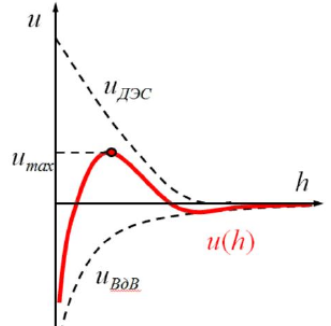
\includegraphics[width=0.3\textwidth]{Images/ДЛФО.png}
    \caption{Зависимость $u(h)$.}
\end{wrapfigure} \;

\begin{itemize}
    \item Силы Ван-дер-Ваальса: $u_{\text{ВдВ}} \sim -\frac{1}{h^2}$
    \item Сила расклинивающего давления: $u_{\text{ДЭС}}  \sim e^{-h/\lambda} $, где $\lambda  = \sqrt{\frac{\varepsilon \varepsilon_0RT}{2F^2I}}$
\end{itemize}

При достаточно высоком заряде поверхности частиц электростатическая энергия отталкивания может преобладать на средних
расстояниях: тогда на
кривой суммарной энергии взаимодействия появляется максимум (потенциальный
барьер), препятствующий агрегации.

\subsection{Типы и правила коагуляции.}\;


Учитывая столь важную
роль электростатических взаимодействий одним из наиболее известных способов коагуляции лиофобных систем является действие растворов электролитов. Согласно
структуре двойного электрического слоя по действию на каждую из его составляющих
различают два типа электролитной коагуляции:
\begin{itemize}
    \item Нейтрализационную (эффективна при низких поверхностных зарядах частиц), обусловленную понижением заряда диспергированных частиц за счет адсорбции на них противоионов;
    \item Концентрационную (эффективна при высоких поверхностных зарядах частиц), обусловленную сжатием двойного электрического слоя (при этом заряд поверхности не меняется).
\end{itemize}
Правила, применимые к коагуляции лиофобных коллоидных систем:
\begin{itemize}
    \item \textbf{Правило Шульце-Гарди.} Коагулирующим действием обладают те ионы электролита-коагулятора, знак заряда которых противоположен заряду частицы дисперсии, а коагулирующее действие возрастает с увеличением заряда иона-коагулятора. Для одно-двух и трехвалентного ионов коагулирующее действие примерно относятся как 1: 50 : 500.
    \item \textbf{Правило Дерягина-Ландау.} При электролитной коагуляции по концентрационному механизму порог коагуляции обратно пропорционален заряду противоионов в шестой степени. 
    \item \textbf{Правило Эйлерса-Корфа.} При нейтрализационной коагуляции порог коагуляции обратно пропорционален второй степени заряда добавляемых противоионов.
\end{itemize}

\subsection{Строение мицелл лиофобных коллоидных растворов.}\;
   \begin{figure}[h!]
	\centering{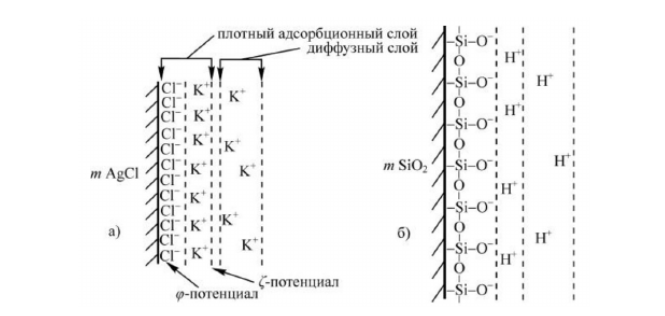
\includegraphics [scale=0.6]{Images/Мицеллы.png}}
        \caption{ДЭС на поверхности коллоидных частиц.}
    \end{figure}
\par У коллоидных частиц поверхностный заряд
обусловлен избирательной адсорбцией ионов, либо диссоциацией поверхностных групп.
Возникающая заряженная
частица, окруженная противоионами называется мицеллой, подобно мицеллам ПАВ.

Как и у поверхности металлических электродов слой противоионов разделяют на две
составляющие – плотную часть, в которой ионы находятся непосредственно у заряженной
поверхности и диффузную часть, где нейтрализующий заряд постепенно спадает в глубь
раствора. Одним
из распространенных методов оценки заряда и потенциала коллоидных частиц является
определение скорости их движения в электрическом поле. Однако в процессе такого
движения двойной электрический слой разрывается. Место разрыва при перемещении
твердой и жидкой фаз друг относительно друга называется плоскостью скольжения. 
Потенциал на плоскости скольжения называют электрокинетическим или дзета-
потенциалом ($\zeta$ -потенциал). Другими словами, $\zeta$ -потенциал – это разность потенциалов в
объеме дисперсионной среды и в плоскости скольжения, т.е. на границе неподвижного
слоя жидкости, окружающего частицу. Важность $\zeta$ -потенциала состоит в том,
что его значение может быть связано с устойчивостью коллоидных дисперсий. Обычно,
устойчивым
коллоидам
соответствует
значение
$\zeta$ -потенциала,
превышающее
по
абсолютной величине 30 мВ. При более низких его значениях коллоидные растворы
подвергаются коагуляции или флокуляции.
 
\section{Ход работы.}
\subsection{Получение золей и исследование их свойств.}
    \begin{enumerate}
    \item \textbf{Получение золя серы $S$ методом замены растворителя.}
    \par Данный способ основывается на том, что раствор становится пересыщенным из-за замены лучшего растворителя на худший. В данном случае ацетон, как неполярный растовритель, заменяется на воду. В таких условиях образуется золь серы $S$ (Рис. 3), который опалесцирует (при проходящем свете окрашивается в жёлтый, а при боковом - в синеватый в результате рассеивания).
    \begin{figure}[!htb] 
        \minipage{0.42\textwidth}
            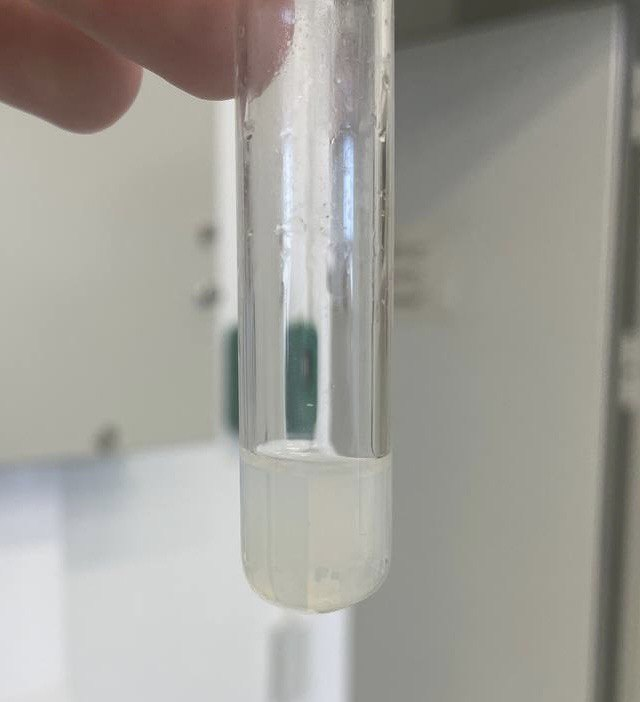
\includegraphics[width=\linewidth]{Images/сера.jpg}
            \caption{Полученный золь серы $S$.}
        \endminipage\hfill
        \minipage{0.4\textwidth}
             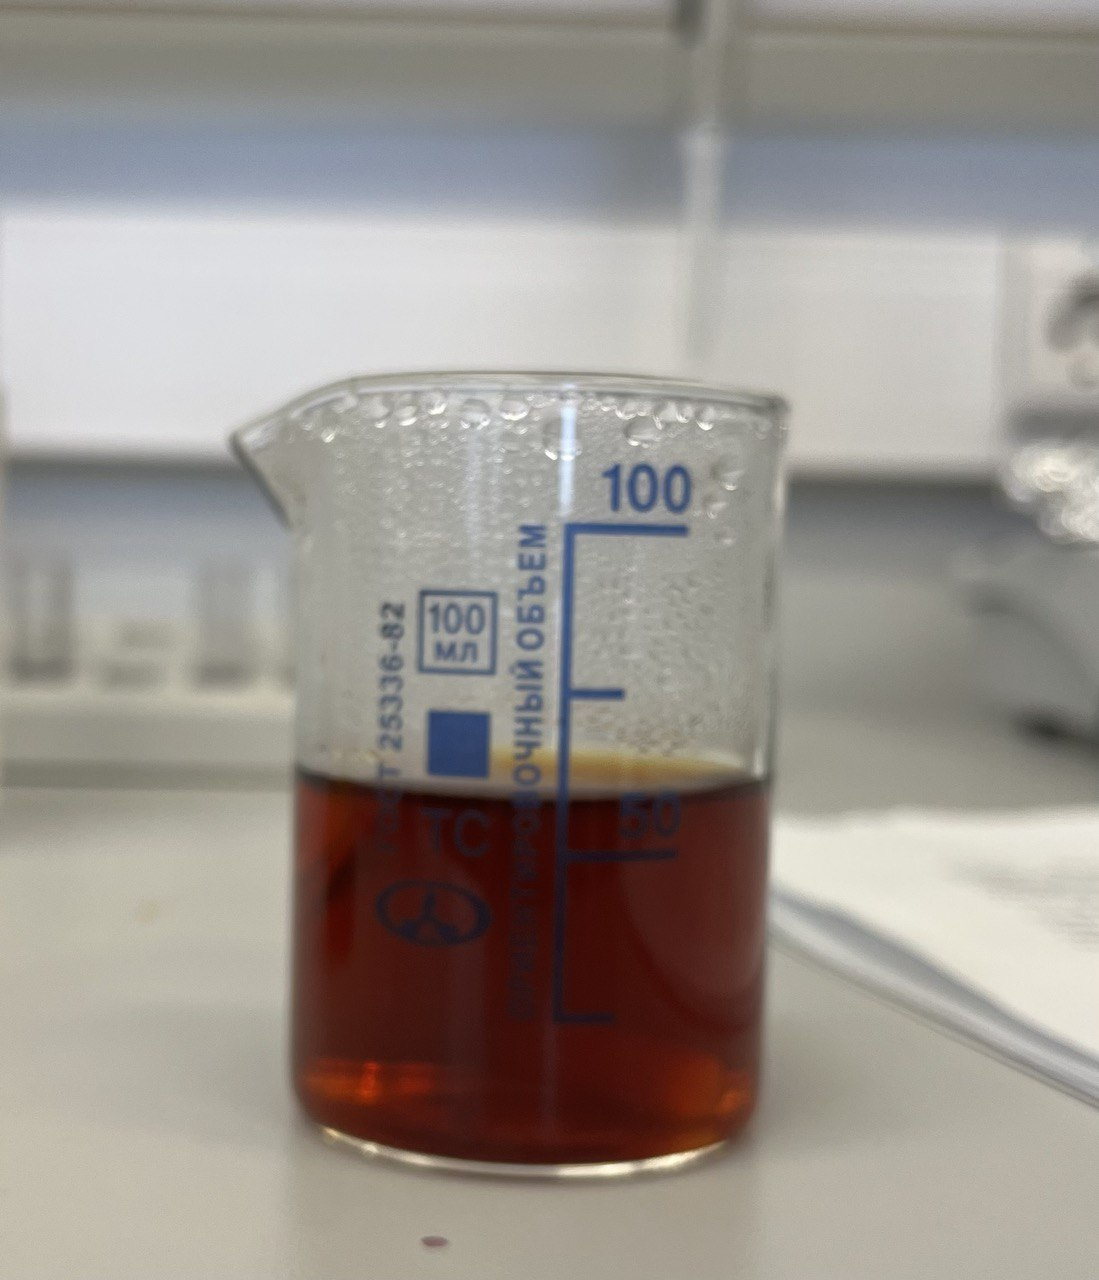
\includegraphics[width=\linewidth]{Images/коньяк.jpg}
              \caption{Полученный золь гидроксида железа $Fe(OH)_3$ методом конденсации.}
        \endminipage
    \end{figure}
    
    \item \textbf{Получение золя гидроксида железа $Fe(OH)_3$ методом конденсации.}
    \par Для получения золя гидроксида железа $Fe(OH)_3$ доводим до кипения 50 мл дистиллированной воды и при перемешивании добавляем 5 мл 2$\%$ раствора $FeCl_{3}$. При этом будет протекать следующая реакция:
    $$\mathrm{FeCl_3 + 3 H_{2}O = Fe(OH)_3 \downarrow}$$
    \par Образуется коллоидный раствор коньячного цвета (Рис. 4), мицеллы представляются формулой:
    $$\mathrm{([m Fe(OH)_3 ] nFeO^+ (n-x)Cl^- )^{x+} xCl^-}$$
    \par Стабилизатором выступает оксохлорид железа (III), образующийся при реакции:
    $$\mathrm{Fe(OH)_3 + HCl = FeOCl + 2 H_{2}O}$$
    \par Правило Панета-Фаянса-Гана объясняет избирательную адсорбцию катионов на поверхности частиц золя: $FeO^{+}$, который находится в большей концетрации, чем $Fe^{3+}$, так же способен достраивать кристаллическую решётку нерастворимого $Fe(OH)_3$, поэтому преимущественно будут образовываться мицеллы именно с $FeO^{+}$.
    \item \textbf{Получение золя гидроксида железа $Fe(OH)_3$ методом пептизации.}

    В стакан отмерим 25 мл дистиллированной воды и 0,5 мл 10$\%$-ного раствора $FeCl_3$. В полученный раствор по каплям добавляем 5$\%$-ный раствор аммиака до тех пор, пока количество образующегося осадка не перестанет увеличиваться. В растворе происходят процессы, описываемые следующей химической реакцией:
    $$FeCl_3 + 3NH_3 \cdot H_2O = Fe(OH)_3\downarrow + 3NH_4Cl$$

    Затем проведём три серии декантации с полученным раствором. После чего к промытому осадку добавим 25 мл дистиллированной воды, взболтаем и, не давая осесть гидроксиду железа, перенесём пипеткой по 2 мл образовавшейся суспензии в 5 чистых пробирок. 

    В каждую из пробирок (кроме контрольной) добавим фиксированный объём пептизатора (10$\%$-ного раствора $FeCl_3$). Энергично перемещаем содержимое и оставим пробирки в штативе на час. В растворах просиходят процессы пептизации и образуются положительно заряженные коллоидные частицы следующего строения:
    $$\{[m Fe(OH)_3] nFe^{3+} 3(n-x)Cl^{-}\}^{3x+}3xCl^{-}$$

    Задетектируем соотношение осадка и раствора в разных пробирках (Рисунки 5, 6, 7, 8 и 9).

    Все полученные сведения занесём в Таблицу 1.

    \begin{table}[h!]
    \caption{Данные по пептизации золя гидроксида железа.}
    \centering
\begin{tabular}{|l|l|l|l|l|l|}
\hline
№ & 1 & 2 & 3 & 4 & 5 \\ \hline
Объём суспензии, мл & 2 & 2 & 2 & 2 & 2 \\ \hline
Объём воды, мл & 5,0 & 4,8 & 4,6 & 4,4 & 4,2 \\ \hline
Объём пептизатора, мл & - & 0,2 & 0,4 & 0,6 & 0,8 \\ \hline
Степень пептизации & - & + & ++ & +++ & ++++ \\ \hline
\end{tabular}
\end{table}
    
     \begin{figure}[!htb] 
        \minipage{0.21\textwidth}
            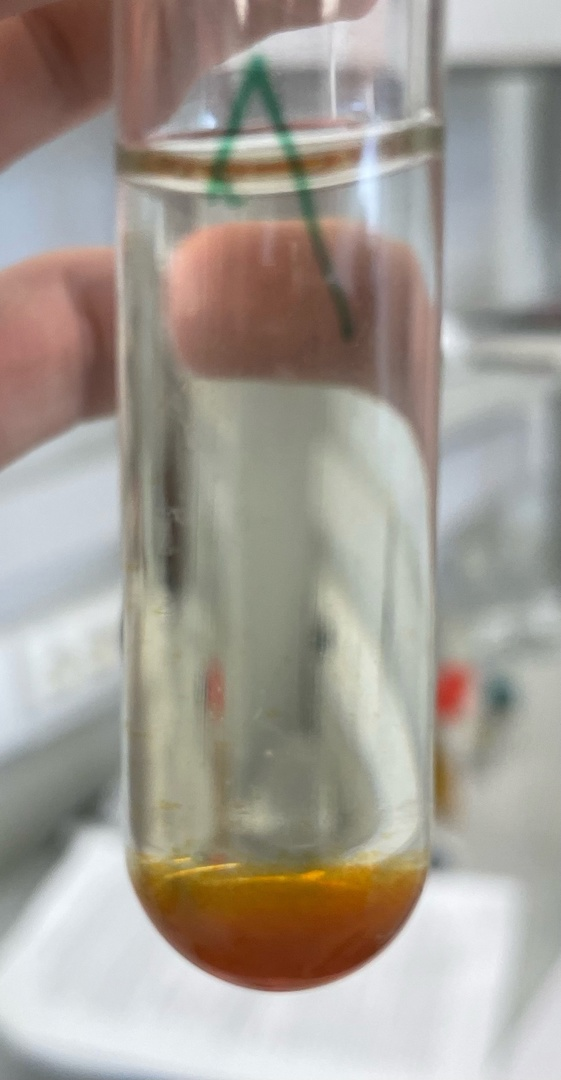
\includegraphics[width=\linewidth]{Images/Пробирка 1.jpg}
            \caption{Пробирка 1.}
        \endminipage\hfill
        \minipage{0.187\textwidth}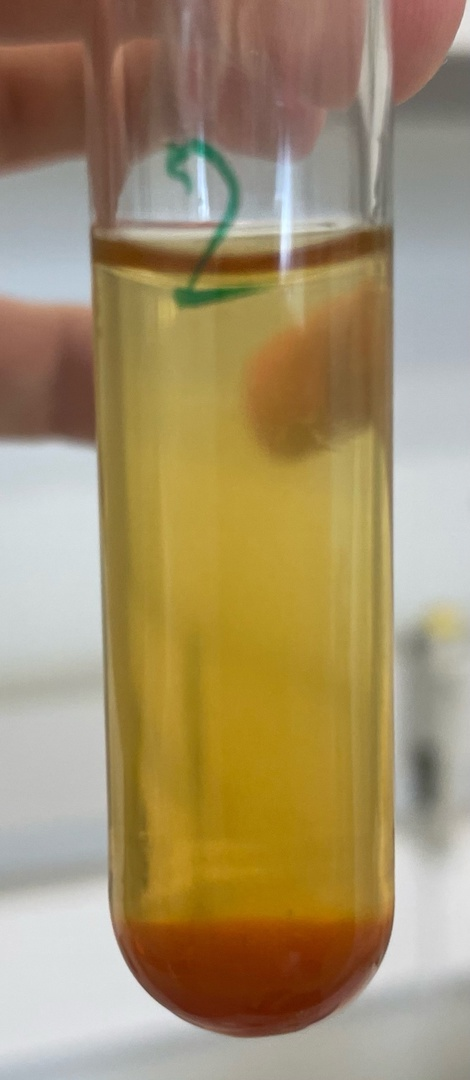
\includegraphics[width=\linewidth]{Images/Прбирка 2.jpg}
            \caption{Пробирка 2.}
        \endminipage\hfill
        \minipage{0.189\textwidth}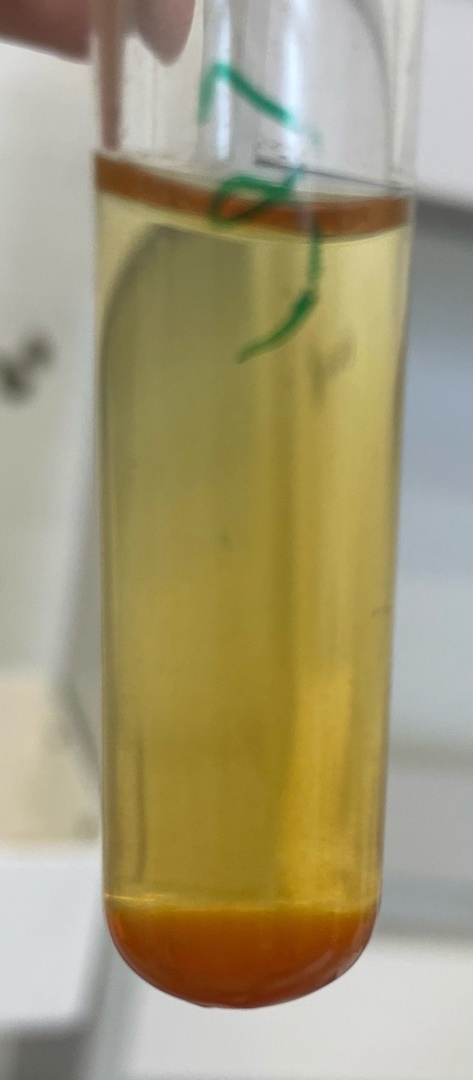
\includegraphics[width=\linewidth]{Images/Пробирка 3.jpg}
            \caption{Пробирка 3.}
        \endminipage\hfill
        \minipage{0.179\textwidth}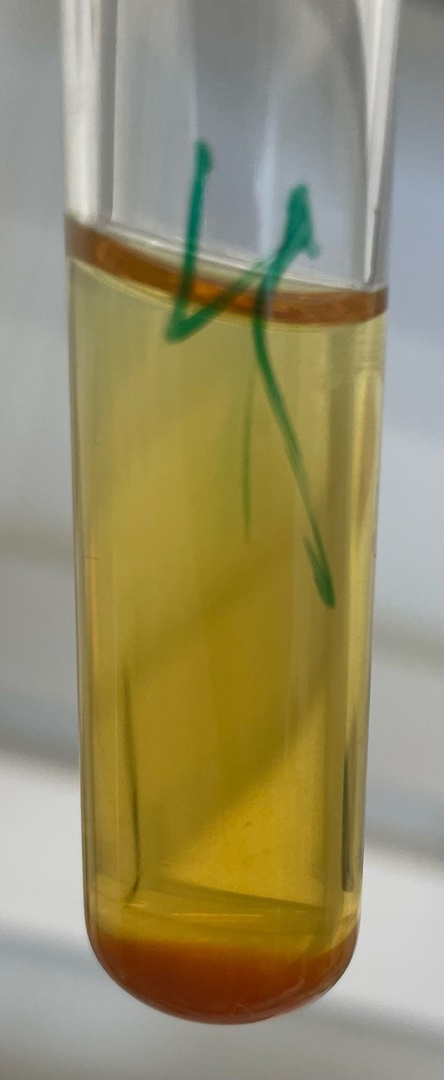
\includegraphics[width=\linewidth]{Images/Пробирка 4.jpg}
            \caption{Пробирка 4.}
        \endminipage\hfill
        \minipage{0.177\textwidth}
             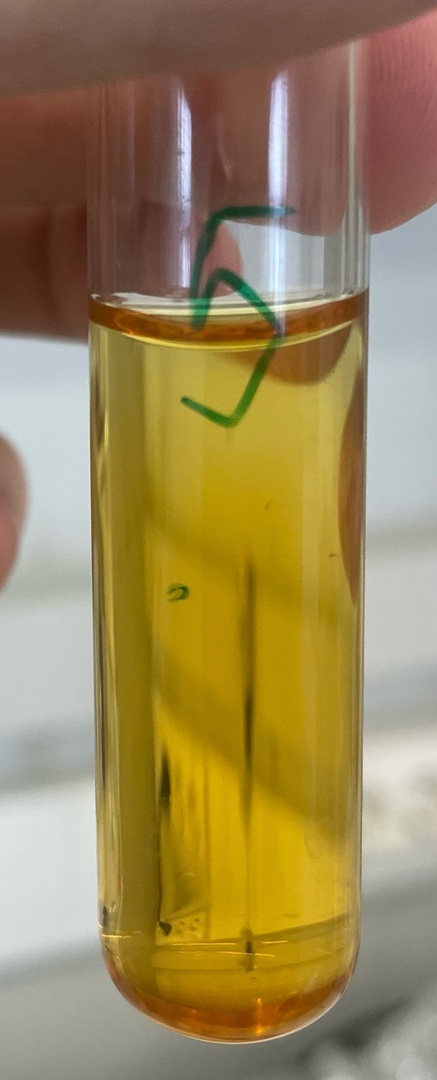
\includegraphics[width=\linewidth]{Images/Пробирка 5.jpg}
              \caption{Пробирка 5.}
        \endminipage
    \end{figure}
    
    \item \textbf{Получение золя Au (по методике Дж. Туркевича и соавторов).} 


    
    В нагретую до кипения дистиллированную воду ($V_{H_2O} = 25 \; \text{мл}$) добавим 250 мкл золотохлористоводородной кислоты $HAuCl_4$ ($1 \; \%$ по массе раствор). Таким образом, можно оценить количество вещества $HAuCl_4$: $\nu_{HAuCl_4} = \frac{V \; \cdot \; \rho \; \cdot \; \omega}{M_{HAuCl_4}} \approx 7,35 \cdot 10^{-6} \; \text{моль}$. Через три минуты кипячения при размещивании быстро добавим 700 мкл раствора цитрата натрия $Na_3Cit$  ($1 \; \%$ по массе). Проведём аналогичный расчёт количества вещества: $\nu_{Na_3Cit} = \frac{V \; \cdot \; \rho \; \cdot \; \omega}{M_{Na_3Cit}} \approx 2,71 \cdot 10^{-5} \; \text{моль}$. Затем при размешивании кипятим смесь 5 - 8 минут до тех пор, пока окраска раствора не перестанет меняться. Полученный золь охлаждаем для последующих исследований.

    Согласно методике напишем суммарную реакцию цитратного восстановления:
    $$2HAuCl_4 + 3Na_3Cit \longrightarrow 2Au + 3Na_2(O = C(CH_2COO)_2) + 3CO_2 + 3NaCl + 5HCl$$

    Учитывая стехиометрию данной химической реакции придём к следующему простому выводу:
    $$\nu_{Na_3Cit}^{react} = \frac{3}{2}\nu_{HAuCl_4} = 11,03 \cdot 10^{-6} \; \text{моль} < 2,71 \cdot 10^{-5} \; \text{моль}$$

    Следовательно, цитрат натрия присутствует в реакционной смеси в избытке. Отсюда вытекает, что на поверхности золота адсорбируются отрицательно заряженные цитрат-ионы, таким образом, порождающие отрицательно заряженные коллоидные частицы Au.

    С помощью спектрофотометра зарегестрируем спектр экстинкции полученного золя в диапазоне длин волн от 300 до 700 нм (Рис. 11).

    \begin{figure}[!htb] 
        \minipage{0.39\textwidth}
            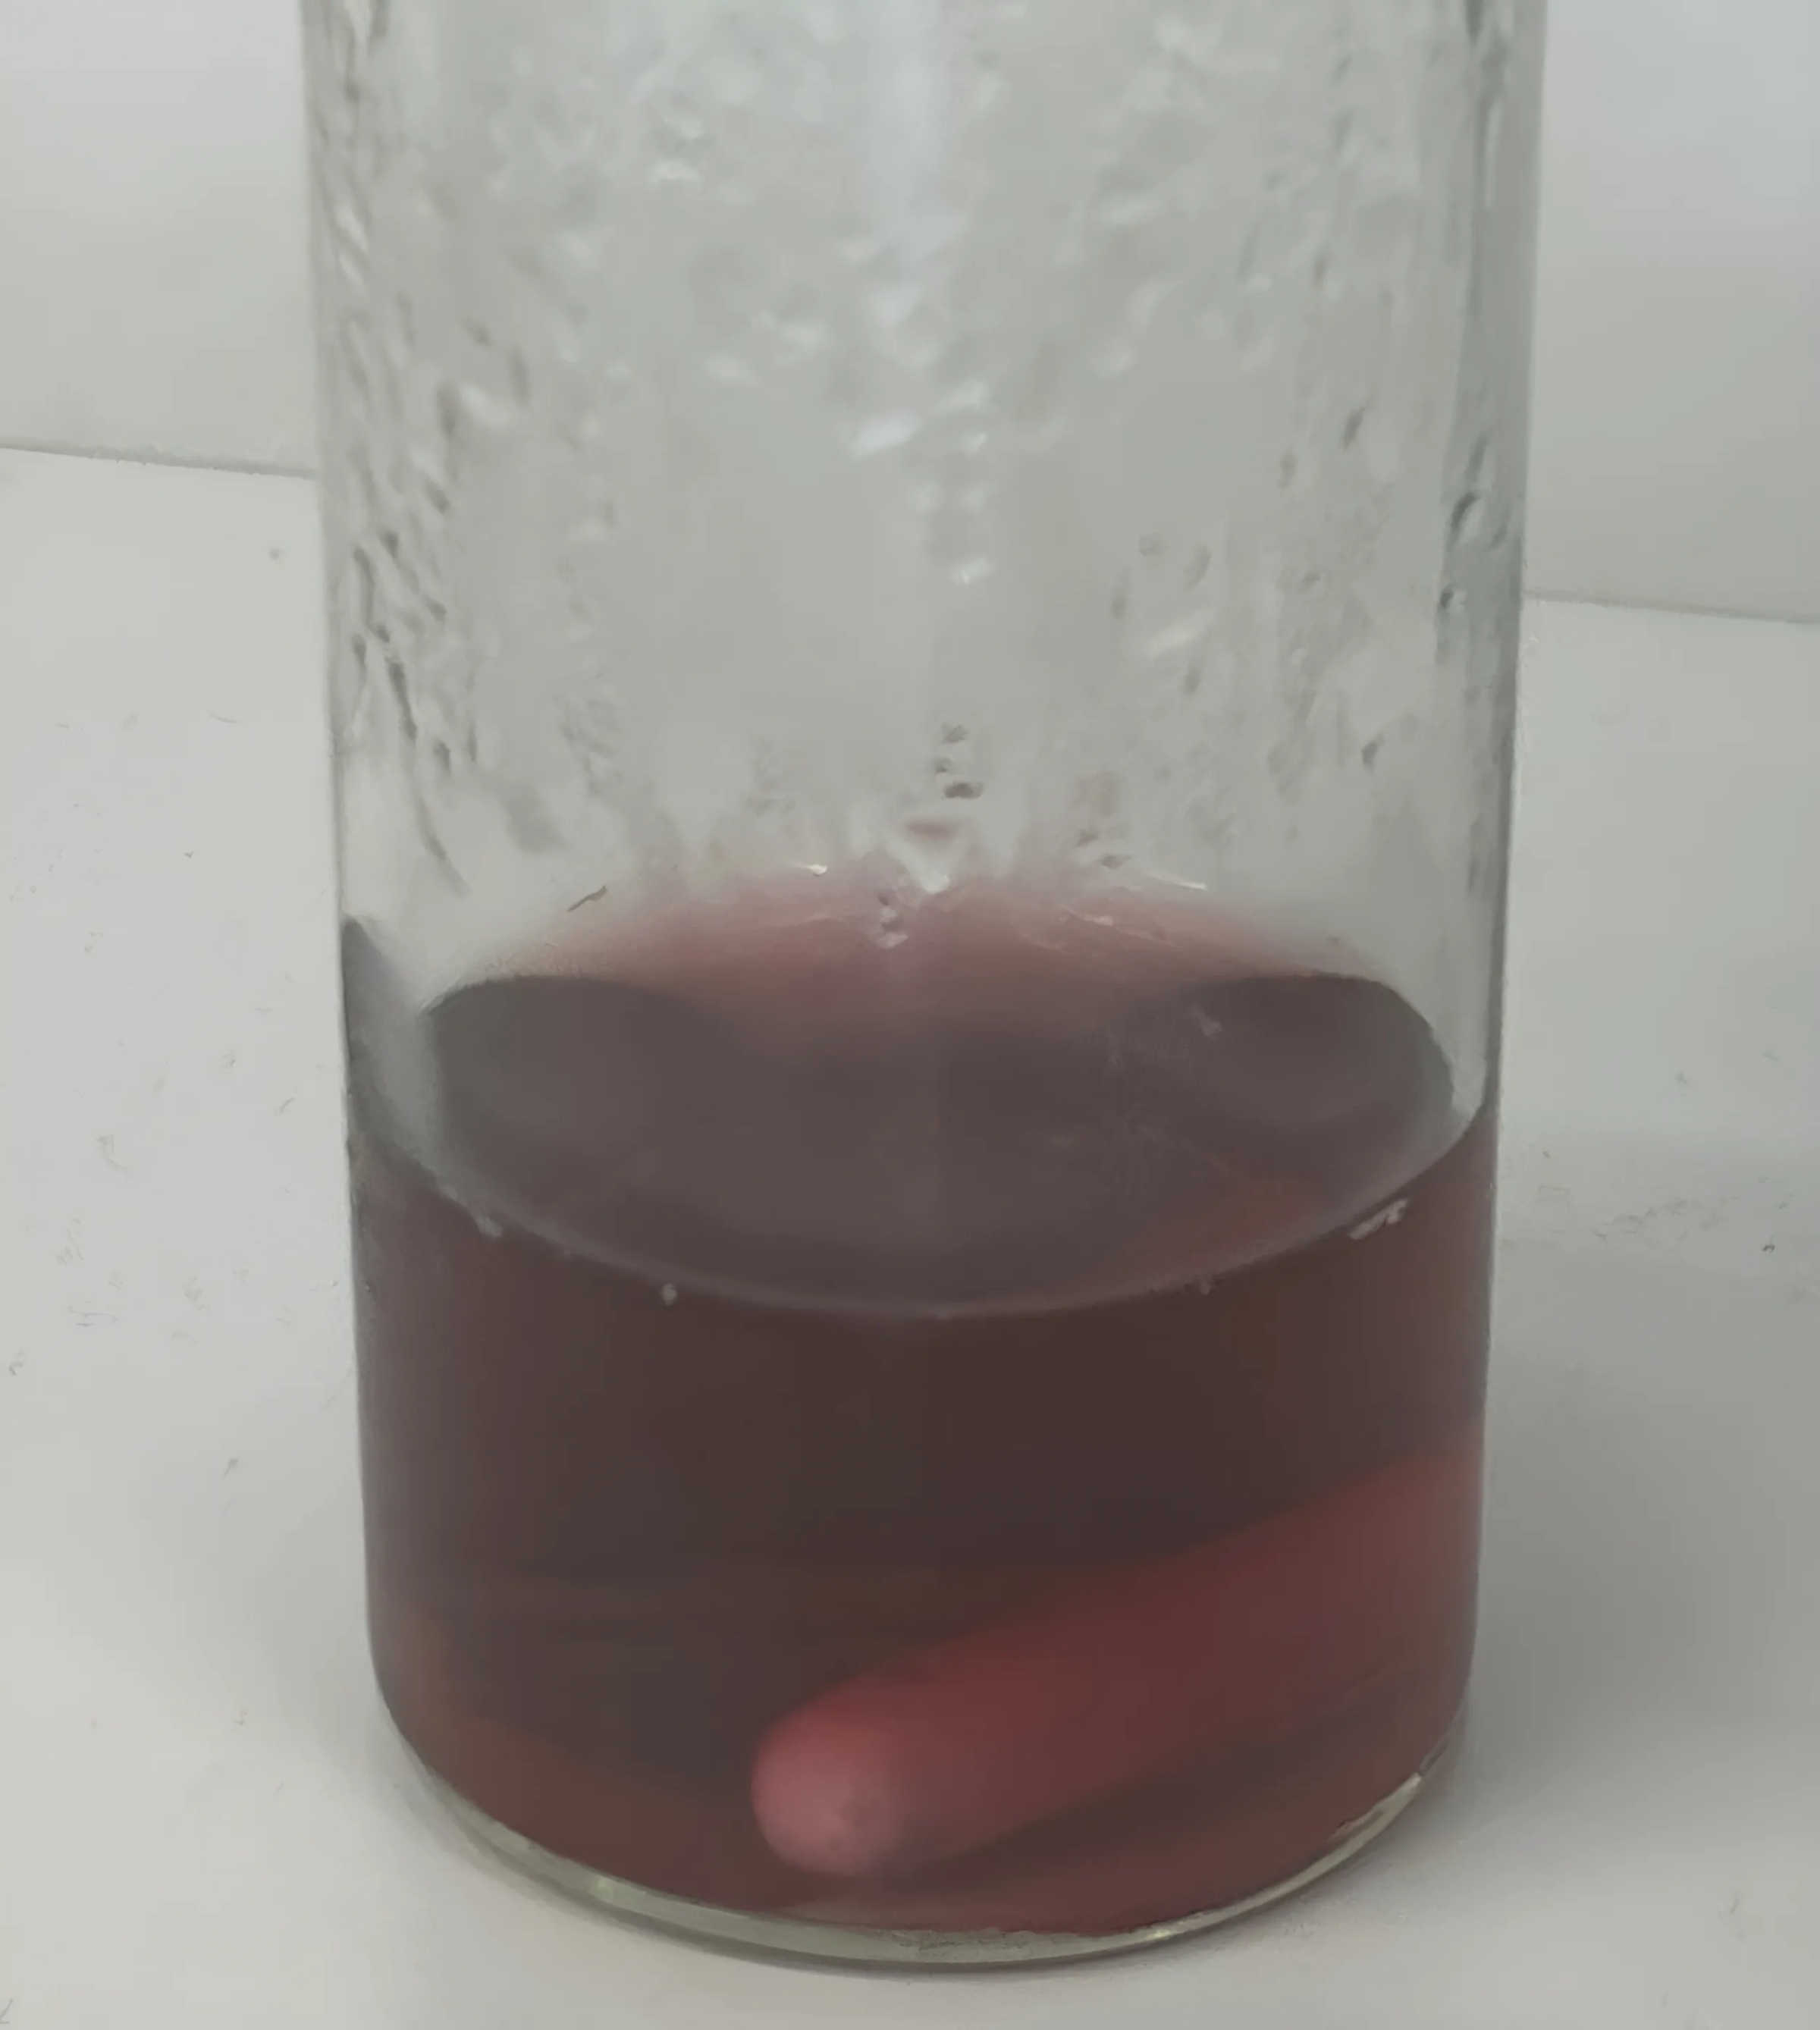
\includegraphics[width=\linewidth]{Images/Золь золота.png}
            \caption{Полученный золь Au.}
        \endminipage\hfill
        \minipage{0.59\textwidth}
             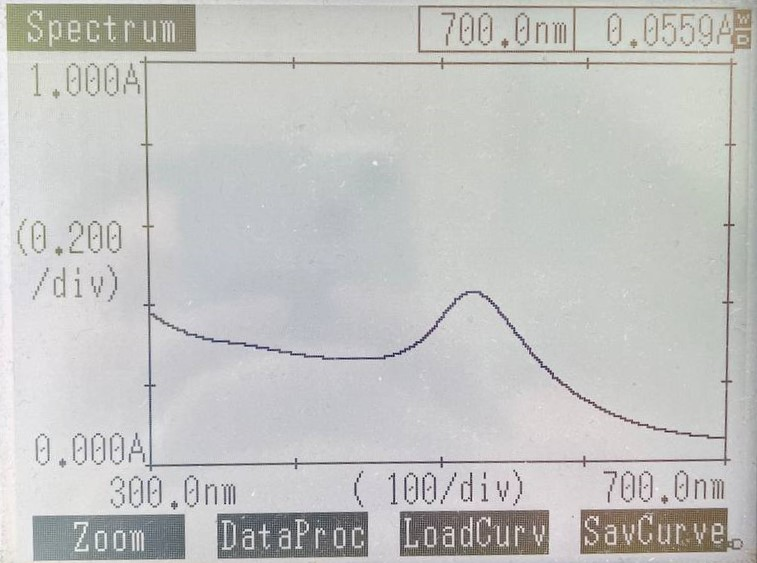
\includegraphics[width=\linewidth]{Images/СПЕКТР МАТЬ ЕГО АДСОРБЦИИ.jpg}
              \caption{Спектр экстинкции.}
        \endminipage
    \end{figure}

    Положение максимума на зарегестрированном спектре: $\lambda^{ext}_{max} = 524,6 \; \text{нм}$. Исходя из полученной величины, определим диаметр золотых частиц двумя способами. Первый, используя соответствующий график зависимости длины волны от диаметра наночастиц (Богатырев В.А., Дыкман Л.А., Хлебцов Н.Г. Методы синтеза наночастиц с плазмонным резонансом. Саратов: Саратовский
    государственный университет им. Н.Г. Чернышевского, 2009), представленный на Рис. 12. Второй способ подразумевает использование аппроксимации этой зависимости по следующей формуле: $\lambda_{max} = 518.8 - 0.0172 \cdot d + 0.0063 \cdot d^2 - 0.0000134 \cdot d^3$ (Njoki P.N. et al. Size Correlation of Optical and Spectroscopic Properties for Gold
    Nanoparticles. J. Phys. Chem. C. 2007 V. 111 P. 14664-14669.). 

    \begin{figure}[!htb] 
        \minipage{0.39\textwidth}
            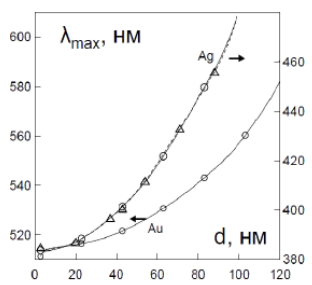
\includegraphics[width=\linewidth]{Images/Способ 1.png}
            \caption{Первый способ.}
        \endminipage\hfill
        \minipage{0.59\textwidth}
             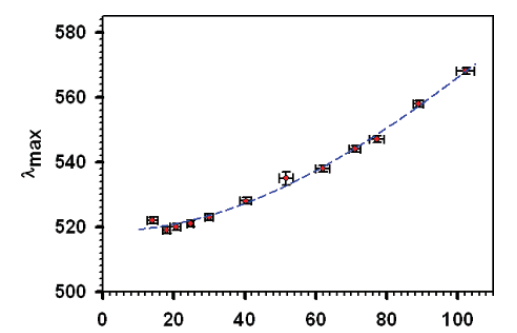
\includegraphics[width=\linewidth]{Images/Способ 2.png}
              \caption{Второй способ.}
        \endminipage
    \end{figure}

    По итогу, получаем следующие значения:
    $$d_1 = 50,2 \; \text{нм}; \; d_2 = 33,0 \; \text{нм}$$

    На основе этих данных оценим верхнюю границу концентрации частиц золота в растворе.

    Для этого в начале определим концентрацию золота в полученном растворе, основываясь на стехиометрии приведённой выше реакции:
    $$C_{Au} = \frac{\nu_{Au}}{V_{sol}} = 2,83 \cdot 10^{-4} \; \text{М}$$

    Количество частиц в растворе найдем, исходя из массы золота и массы одной частицы, посчитанной по размерам частиц и плотности золота:
    $$N = \frac{m}{m_{\text{ч}}} = \frac{1,45 \cdot 10^{-3}}{3,64 \cdot 10^{-16}} = 3,99 \cdot 10^{12} \; \text{частиц}$$

    В конце концов, определим концентрацию частиц в объёме:
    $$C_{\text{ч}} = 1,54 \cdot 10^{17} \; \frac{\text{частиц}}{\text{м}^3}$$

    Согласно теории Смолуховского, рассчитаем константу быстрой коагуляции и время полупревращения:
    $$k = \frac{8}{3} \frac{k_b T}{\eta} = 1,07 \cdot 10^{-17} \; \frac{\text{м}^3}{c}$$
    $$\tau = \frac{1}{k \cdot n} = 0,61 \text{с}$$
    \end{enumerate}

    \subsection{Определение порогов коагуляции золей.}
    \par В этой части работы исследования проводились с золем золота $Au$, приготовленным в предыдущем пункте. Определение порога быстрой коагуляции золя по отношению к разным электролитам (0.5M $KNO_{3}$, 0.01M $Mg(NO_{3})_{2}$, 0.001M $K_{3}[Fe(CN)_{6}]$) устанавляивается по изменению цвета раствора с вишнёвого на синеватый. Фиксируется минимальная концетрация электролита, при которой это происходит мгновенно (Таблица 2).
    \begin{table}[!h]
    \centering
    \begin{tabular}{|l|l|l|l|l|}
    \hline
    
    Соль & $V_{\textbf{эл-та}}$, мкл & C $\cdot 10^{-3}$, М& ln(C)      & ln(Z)      \\ \hline
    $KNO_3$ & 225 & 56,25 & -2,8779 & 0 \\ \hline
    $Mg(NO_3)_3$ & 345 & 1,725 & -6,3625 & 0,693147 \\ \hline
    $La(NO_3)_3$ & 688 & 0,344 & -7,9749 & 1,098612       \\ \hline
    \end{tabular}
    \caption{Пороги коагуляции солей}
    \label{tab2}
    \end{table}
    \par По полученным значениям построим график (Рис. 14) в двойных логарифмических координатах, чтобы определить степень ($n$) в зависимости $C \sim \dfrac{1}{z^n}$.
        \begin{figure}[h!]
	\centering{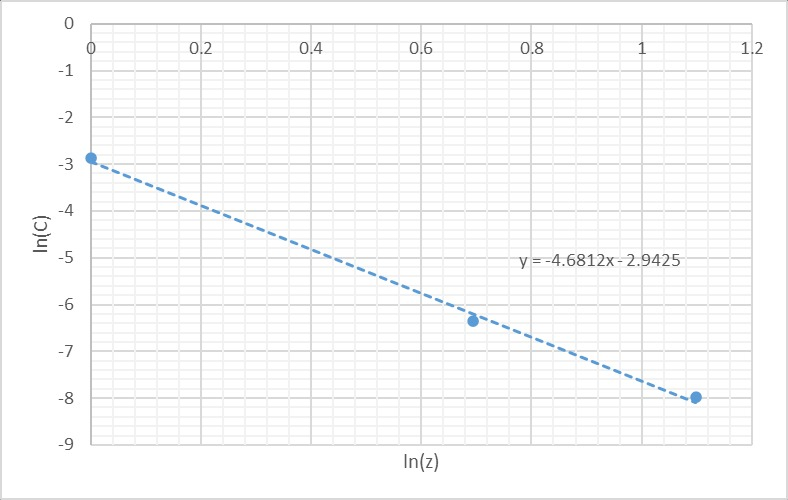
\includegraphics [scale=0.5]{Images/порог.jpg}}
        \caption{График зависимости порога коагуляции от заряда катиона электролита.}
    \end{figure}
    \par Из угла наклона определяем, что зависимость $C \sim \dfrac{1}{z^\text{4,68}}$, следовательно преобладает концетрационный механизм коагуляции согласно правилу Дерягина-Ландау.
    \section{Выводы.}
    \begin{itemize}
        \item Согласно методике был получен золь серы $S$ методом замены растворителя. Наблюдалось явление опалесценции.
        \item Согласно методике был получен золь гидроксида железа $Fe(OH)_3$ методом конденсации. Наблюдался эффект Тиндаля, так же было предположено объяснение избирательной адсорбции согласно правилу Панета-Фаянса-Гана.
        \item В ходе исследования зависимости степени пептизации коллоидного раствора, на примере образования золя гидроксида железа $Fe(OH)_3$, было установлено, что данный параметр зависит от концентрации пептизатора в растворе и увеличивается по мере увеличения добавленного объёма раствора $FeCl_3$.
        \item Используя полученный по методике золь золота, с помощью спектра экстинкции смогли оценить размер частиц золота в коллоидном растворе ($d_2 = 33,0 \; \text{нм}$) и их концентрацию ($C_{\text{ч}} = 1,54 \cdot 10^{17} \; \frac{\text{частиц}}{\text{м}^3}$), используя известные формулы и источники, указанные в тексте. Также по модели Смолуховского рассчитали константу скорости быстрой коагуляции полученного золя ($k = 1,07 \cdot 10^{-17} \; \frac{\text{м}^3}{c}$) и время, за которое количество исходных частиц (мономеров) уменьшится вдвое ($\tau = 0,61 \text{с}$).
        \item Были определены пороги быстрой коагуляции золя золота $Au$ по отношению к разным электролитам. Из этих данных было установлено несильное преобладание концетрационного механизма коагуляции с зависимостью $C \sim \dfrac{1}{z^\text{4,68}}$.
    \end{itemize}
\end{document}
